\section{Технический проект}
\subsection{Общая характеристика организации решения задачи}

Необходимо спроектировать и разработать приложение, которое должно способствовать продвижению компании на рынке.

Игровой движок -- базовое ПО компьютерной игры, которое пригодно для повторного использования и расширения, и тем самым может быть рассмотрено как основание для разработки множества различных игр без существенных изменений. В дополнение к многократно используемым программным компонентам, игровые движки предоставляют набор визуальных инструментов для разработки. Эти инструменты обычно составляют интегрированную среду разработки для упрощённой, быстрой разработки игр на манер поточного производства.

\subsection{Обоснование выбора технологии проектирования}

На сегодняшний день информационный рынок, поставляющий программные решения в выбранной сфере, предлагает множество продуктов, позволяющих достигнуть поставленной цели – разработки игрового приложения.

\subsubsection{Описание используемых технологий и языков программирования}

В процессе разработки игрового движка используются программные средства и языки программирования. Каждое программное средство и каждый язык программирования применяется для круга задач, при решении которых они необходимы.

\subsubsection{Язык программирования C\#}

C\# - объектно-ориентированный язык программирования общего назначения. Разработан в 1998—2001 годах группой инженеров компании Microsoft под руководством Андерса Хейлсберга и Скотта Вильтаумота как язык разработки приложений для платформы Microsoft .NET Framework и .NET Core. Впоследствии был стандартизирован как ECMA-334 и ISO/IEC 23270.
C\# относится к семье языков с C-подобным синтаксисом, из них его синтаксис наиболее близок к C++ и Java. Язык имеет статическую типизацию, поддерживает полиморфизм, перегрузку операторов (в том числе операторов явного и неявного приведения типа), делегаты, атрибуты, события, переменные, свойства, обобщённые типы и методы, итераторы, анонимные функции с поддержкой замыканий, LINQ, исключения, комментарии в формате XML.
На сегодняшний момент язык программирования C\# один из самых мощных, быстро развивающихся и востребованных языков в ИТ-отрасли. В настоящий момент на нем пишутся самые различные приложения: от небольших десктопных программок до крупных веб-порталов и веб-сервисов, обслуживающих ежедневно миллионы пользователей.
C\# является объектно-ориентированным и в этом плане много перенял у Java и С++. Например, C\# поддерживает полиморфизм, наследование, перегрузку операторов, статическую типизацию. Объектно-ориентированный подход позволяет решить задачи по построению крупных, но в тоже время гибких, масштабируемых и расширяемых приложений. И C\# продолжает активно развиваться, и с каждой новой версией появляется все больше интересных функциональностей.

\paragraph{Роль платформы .NET}

Когда говорят C\#, нередко имеют в виду технологии платформы .NET (Windows Forms, WPF, ASP.NET, .NET MAUI). И, наоборот, когда говорят .NET, нередко имеют в виду C\#. Однако, хотя эти понятия связаны, отождествлять их неверно. Язык C\# был создан специально для работы с фреймворком .NET, однако само понятие .NET несколько шире.
Фреймворк .NET представляет мощную платформу для создания приложений. Можно выделить следующие ее основные черты:
\begin{enumerate}
	\item Поддержка нескольких языков.
	\item Кроссплатформенность.
	\item Мощная библиотека классов.
	\item Разнообразие технологий.
	\item Производительность.
\end{enumerate}

\paragraph{Преимущества использования и изучения C\#}

C\# является управляемым языком программирования, что позволяет разработчику не следить за выделением и использованием памяти. Для этого существует CLR (Common Language Runtime) – виртуальная машина, которая занимается запуском приложения, а также управлением памятью.
Также C\# является строго типизированным и объектно ориентированным языком, что позволяет использовать ООП в его классическом виде. Здесь нет множественного наследования классов, что упрощает понимание ООП, но есть множественная реализация интерфейсов, что дает большую гибкость для разработчиков.
Большое сообщество и универсальность языка дают большое поле для деятельности. Как уже было указано ранее, вы можете разрабатывать веб-приложения, сложные микросервисные платформы, игры, а так же мобильные приложения. Здесь действительно серьезный инструментарий для разработки, такие IDE как Visual Studio или JetBrains Rider. Наличие огромнейшего разнообразия библиотек на все случаи жизни, от обратки изображений и видео, до нейросетей. А кроссплатформенность дает возможность писать код как на Windows, так и на macOS и Linux.
Как уже было сказано ранее, C\# является языком программирования общего назначения, а значит покрывает большое количество задач и областей, а именно:
\begin{enumerate}
	\item Web – разработка web-приложений и сервисов для платформ macOS, Windows, Linux и Docker.
	\item Mobile – разработка единой кодовой базы для построения нативных приложения для iOS и Android.
	\item Desktop – разработка нативных приложения под Windows и macOS.
	\item Microservices – разработка независимых компонентов запускаемы в Docker контейнерах.
	\item Cloud – использование существующих облачных решений или создание собственных. C\# поддерживается большинством облачных платформ, такими как Azure и AWS.
	\item Machine learning – разработка приложений искусственного интеллекта и машинного обучения, решающие проблемы машинного зрения, обработки речи, моделей предсказания, и тд.
	\item Game development – разработка 2D и 3D игра для самых популярных десктопных и мобильных платформ.
	\item Internet of Things (IoT) – разработка приложений для интернета вещей, имеющие поддержку Rasbery Pi и других одноплатных компьютеров.
\end{enumerate}

Исходя из вышеперечисленных областей применения видно, что платформа .NET и язык программирования C\# покрывают большой спектр проектов на рынке. Это говорит нам о том, что изучив язык программирования C\# с легкостью можно найти проект на любой вкус.

\paragraph{Описание движка}
AdventureGame - главный класс движка. Создается класс-наследник MyGame. Здесь будут храниться глобальные переменные конкретной игры (например флаги каких-то событий или квестов). Все функции движка там: добавить комнату, перейти в комнату, поместить персонажа/предмет, установить главного персонажа, удалить персонажа, предмет, запустить/остановить сценарий, передать управление в другой сценарий, разговор персонажа, взять предмет.
То есть это все то, что должно быть доступно в любом сценарии. Поэтому, надо делать класс AdventureGame статическим.Саму игру мы задаем в конструкторе это класса как множество комнат. 

Комната (Room) представляет собой совокупность объектов, а также хранит свою графику. Каждый объект может иметь свой небольшой управляющий сценарий. Эти сценарии работают параллельно, например, несколько объектов могут двигаться одновременно, или происходит одновременная анимация (качается дерево). В этих же сценариях можно управлять звуком (в будущем). Каждый сценарий запускается один раз и далее повторяется в цикле.Комната имеет отдельные сценарии для входа и выхода (то есть запускается один раз при входе героя в комнату и при выходе).К комнатам идет обращение по имени (задается при добавлении комнаты в движок).
Сценарий входа в комнату может проверять какие-то игровые ситуации и настраивать комнату перед отображением. Сценарий выхода может останавливать какие-то вещи.
Каждый объект в комнате имеет имя и сценарий по взаимодействию с ним по клику мыши (например открыть дверь).Также есть еще сценарий, когда герой пересекает объект (подходит к объекту). Здесь происходит перемещение персонажа в другую комнату (указывается в какую комнату). В другой комнате аналогично настроен сценарий на обратный проход (там другая дверь, другой объект).

Персонажи (Actor) имеют свою анимацию движения по комнате. По клику мыши в точку X,Y (или по программно заданным координатам) происходит автоматическое движение.
В комнате также задаются области (как множество прямоугольников), где происходит движение персонажей. Например, если в комнате в центре препятствие, то нужно 4 прямоугольника. Каждый прямоугольник должен касаться друг друга и не должен пересекаться с другими.
Каждый персонаж Actor может иметь набор предметов или инвентарь.

Текст добавляется методом SayLine (например в сценарии взаимодействия).
Объекты расставляются в комнате по координатам. При взаимодействии с объектом персонаж находится в определенном месте (эта позиция задается для объекта) - например, с левой стороны двери. Состояние персонажа (куда он смотрит после того как подошел в заданную позицию) задается в сценарии взаимодействия (запускается после того как персонаж пришел в заданную позицию).
Объект может иметь несколько состояний (одно минимум). Каждое состояние сопоставлено с о спрайтом или анимацией. Например, закрытая и открытая дверь.
Взять объект - PickUpObject - объект попадает в хранилище персонажа.

Анимацию задаем как последовательность кадров с заданной скоростью.
Автоматическое движение объекта задаем в сценарии.

Сценарий запускается (StartScript), и затем работает до тех пор пока не будет остановлен (StopScript).
В сценарии задаем шаги движения, между которыми вызываем Yield (передать управление другому потоку). То есть сценарии - это параллельные потоки.
Глобальные переменные могут быть в классе конкретной игры или в статическом классе Globals. Чтобы к ним обратиться, функция сценария должна также быть в классе игры. Локальные переменные могут быть внутри конкретной комнаты, тогда локальные сценарии находятся в классе комнаты.

Сценарий - это любой метод (например у MyGame или у конкретной комнаты (класса, потомка от Room).
То есть мы в движок передаем метод (через делегат), а уже сам движок делает все что нужно (запускает поток).
У наследника указываются только свои поля. Сценарии размещаются в зависимости от того, что там делается.
Если просто перемещение, смена состояния, смена комнаты - тогда в классе конкретной комнаты (потомка Room).

Отрисовка всех объектов происходит с помощью таймера и события Form\_Paint. Таймер обращается к GraphicsManager, который меняет состояние объектов когда это нужно. Это происходит каждый тик таймера. Затем событие Form\_Paint с помощью Graphics отображает измененные объекты на форме. На выходе мы получаем актуальное состояние каждого объекта, которое можем наблюдать в реальном времени. Это может быть анимация перемещения, появления или исчезновения объекта.


\subsection{Диаграмма компонентов классов}

Диаграмма компонентов описывает особенности физического представления разрабатываемой системы. Она позволяет определить архитектуру системы, установив зависимости между программными компонентами, в роли которых может выступать как исходный, так и исполняемый код. Основными графическими элементами диаграммы компонентов являются компоненты, интерфейсы, а также зависимости между ними. На рисунке \ref{diagram:image} изображена диаграмма компонентов для проектируемой системы. Она включает в себя основной класс движка игры AdventureGame и производные от него классы, класс Object с наследниками и их параметрами (полями и методами).

\begin{figure}[ht]
\center{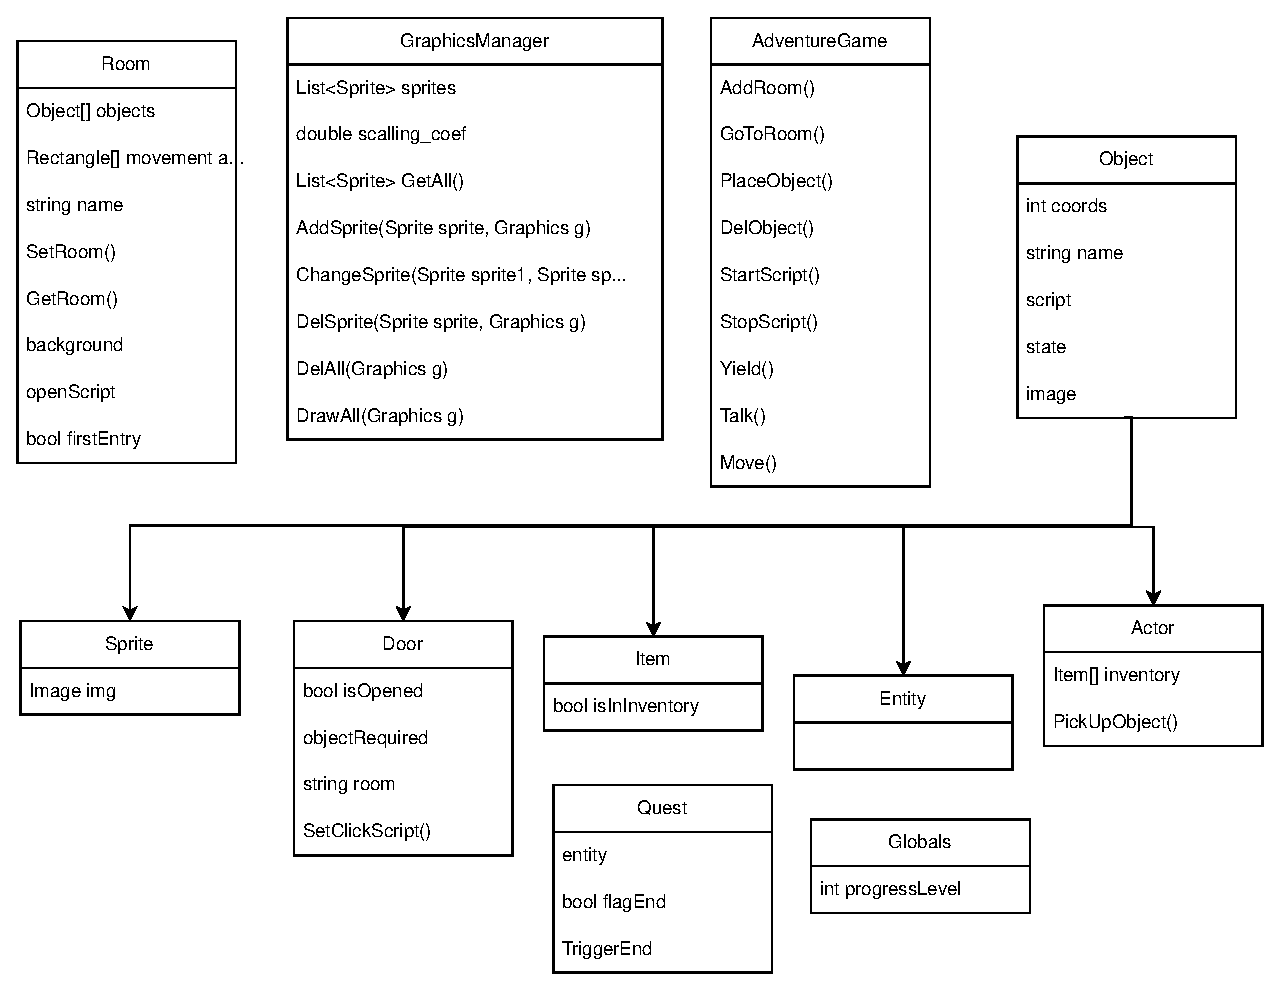
\includegraphics[width=1\linewidth]{diagram}}
\caption{Диаграмма компонентов}
\label{diagram:image}
\end{figure}

\subsection{Описание классов}

\begin{enumerate}
	\item[GraphicsManager] - класс, управляющий спрайтами. Содержит в себе:
	\begin{itemize}
		\item List<Sprite> sprites - список спрайтов;
		\item double scalling\_coef - коэффициент приближения;
		\item AddSprite(Sprite sprite, int x, int y) - добавляет в список спрайт, сохраняет координаты;
		\item ChangeSprite(Sprite sprite1, Sprite sprite2) - меняет местами спрайты в списке;
		\item DelSprite(Sprite sprite) - удаляет спрайт из списка;
		\item DelAll() - очищает список спрайтов;
		\item UpdateGraphics(Graphics g) - с помощью Graphics добавляет все спрайты из списка на форму.
	\end{itemize}
	\item[Sprite] - класс, хранящий в себе изображения игровых объектов Image img.
	\item[Object] - абстрактный класс, от которого наследуются классы Sprite, Item, Entity, Actor, Door.
	\item[Entity] - класс сущностей. Потомок класса Object. Сущность - игровой объект, который считается одушевленным, то есть с ним можно поговорить и нельзя подобрать в инвентарь, в отличие от объекта Item.
	\item[Item] - класс предметов. Предмет - это игровой объект, который является неодушевленным, то есть вещью, которую можно взять в инвентарь. С вещью нельзя разговаривать, в отличие от объекта класса Entity, но она также является потомком класса Object.
	\item[Actor] - главный персонаж игры, которым управляет пользователь. Именно он находится в центре сюжета. Является наследником Object, так как имеет схожие свойства.
	\item[Door] - еще один наследник класса Object. Является по своей сути объектом, реализующим переход между комнатами(Room).
	\begin{itemize}
		\item bool isOpened - состояние двери (открыта/закрыта);
		\item objectRequired - условия, необходимые для того, чтобы дверь открылась. Проверяются при нажатии на дверь;
		\item string name - название комнаты, в которую ведет дверь;
		\item SetClickScript() - события, которые произойдут, когда польователь кликнет на дверь;
	\end{itemize}
	\item[Room] - комната(подлокация), в которой происходит сюжетное действие и игровой процесс. Содержит следующие поля и методы:
	\begin{itemize}
		\item Object[] objects - список всех объектов, которые размещены в данной комнате;
		\item Rectangle[] moveArea - область, по которой может перемещаться персонаж (Actor). Определяется набором прямоугольников, которые не должны пересекаться;
		\item string name - название комнаты;
		\item bool firstEntry - показывает, находится ли персонаж в данной комнате впервые;
		\item SetRoom(string roomName) - устанавливает комнату со всеми ее объектами и их состояниями;
		\item GetRoom(string roomName) - получает комнату со всеми ее объектами и их состояниями;
	\end{itemize}
	\item[Globals] - в данном классе находятся глобальные переменные (флаги) текущей игры. Например, int progressLevel в виде простого числа показывает прогресс игрока в игре.
	\item[AdventureGame] - абстрактный класс, управляющий игрой. Имеет следующие методы:
	\begin{itemize}
		\item AddRoom(string roomName) - добавить комнату;
		\item GoToRoom(string roomNAme) - перейти в комнату;
		\item PlaceObject(Object object, int x, int y) - поместить объект на карту по координатам x и y;
		\item DelObject(Object object) - удалить объект;
		\item StartScript(???) - запускает скрипт;
		\item StopScript(???) - останавливает скрипт;
		\item Yeild(???) - передает управление другому скрипту;
		\item Talk(???) - говорить с персонажем. Отображает текст в текстовом поле внизу экрана. 
		\item Move() - перемещение объектов.
	\end{itemize}
\end{enumerate}



